\documentclass[a4paper]{article}
\usepackage[a4paper,margin=25mm]{geometry}
\usepackage{graphicx,subcaption}
\usepackage{amsmath,amsfonts}
\usepackage{qtree}
\usepackage{tikz}
\title{Notes on Sequence Modelling}
\author{G.A. Jarrad}
\usepackage{accents}
\newcommand{\rvec}[1]{\accentset{\leftarrow}{#1}}
\newcommand{\Bb}[1]{%
  \expandafter\def\csname#1#1\endcsname%
  {\ensuremath{\mathbb #1}}}
\Bb X\Bb S


\begin{document}
\maketitle
\numberwithin{equation}{section}
\numberwithin{figure}{section}
\numberwithin{table}{section}
\section{Random Sequence Processes}
\label{sec:random-processes}
Consider a random process $R$, graphically depicted in Figure~\ref{fig:R-process}, that generates arbitrary sequences of values
of the form $\vec{r}_n=(r_1,r_2,\ldots,r_n)$, where the length of any particular sequence is 
governed by a random variable $N$. Let $\vec{R}_N=(R_1,R_2,\ldots,R_N)$ denote
the corresponding sequence of random variables, where $R_t$ denotes the $t$-th discrete stage in the sequence.
\begin{figure}[hbt]
\centering
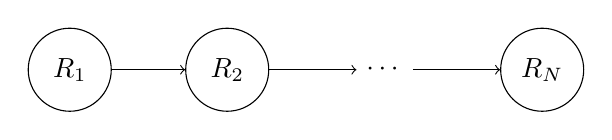
\begin{tikzpicture}[cnode/.style={draw,circle,minimum size=3em,inner sep=3pt}]
    \node[cnode] (1) at (0,0) {$R_1$};
    \node[cnode] (2) at (2, 0)  {$R_2$};
    \node (t) at (4, 0) {$\cdots$};
    \node[cnode] (n) at (6, 0)  {$R_N$};

    \draw[->] (1) edge (2) ;
    \draw[->] (2) edge (t) ;
    \draw[->] (t) edge (n) ;
\end{tikzpicture}
\caption{\em A random process $R$ for generating sequences of arbitrary length $N$. The arrows indicate transitions from one stage in the sequence to the next.}
\label{fig:R-process}
\end{figure}

We assume that each $R_t$ randomly takes some discrete or continuous value $r_t\in{\cal R}$,
and hence the probability (or probability density) of observing a particular
sequence $\vec{r}_n$ of length $n$ is given by
\begin{eqnarray}
   p(\vec{R}_N\!=\!\vec{r}_n) & = & p(N=n)\; p(\vec{R}_n\!=\!\vec{r}_n)\,,
\end{eqnarray}
where
\begin{eqnarray}
p(\vec{R}_n\!=\!\vec{r}_n) & = & p(R_1\!=\!r_1,\ldots,R_n\!=\!r_n)\,.
\end{eqnarray}
In practice, this definition presupposes that we know we have observed a {\em complete} sequence that was initiated
at stage 1 and terminated at stage $n$.
Suppose instead that the sequence $\vec{r}_n$ was observed one stage at a time. How do we know if the
underlying process has actually terminated, or will instead
continue to generate another observed value
$r_{n+1}$, leading to the extended sequence $\vec{r}_{n+1}$? 
Similarly, how do we know that the first observed value $r_1$ was not in fact
part of a longer, unobserved sequence of values $(\ldots,r_0,r_1,\ldots)$?

In order to handle such difficulties, we consider any arbitrary sequence $\vec{r}_n$ to be {\em incomplete},
and explicitly denote the corresponding, complete sequence as $\langle\vec{r}_n\rangle$.
Additionally, we introduce the notion of {\em partially complete} sequences, 
defining a {\em start sequence} to be a sequence that has a definite start but an indefinite end,
denoted by $\langle\vec{r}_n]$, and futher defining an {\em end sequence} to be a sequence
that has a definite end but an indefinite start, denoted by $[\vec{r}_n\rangle$.

Under this augmented notation, knowledge about the start of a sequence can be encapsulated in 
a random indicator variable $\iota_t$, which takes on the value 1 if $R_{t+1}$ is definitely the first stage in the
sequence, or the value 0 if it is not. Similarly, the random indicator variable $\tau_{t}$
takes on the value 1 if $R_{t-1}$ is definitely the last stage in the sequence, or the value 0 if it is not.
We assume that the random process $R$ only ever produces complete sequences described by $\langle\vec{R}_N\rangle$,
independently of the observation process, which might provide partial or complete sequences of values.
Notionally, the indicators $\iota_0$ and $\tau_{N+1}$ can be thought to correspond to pseudo-stages 0 and $N+1$, such that
the generated sequence $\langle\vec{R}_N\rangle$ is initiated at stage 0 and terminated at stage $N+1$.
This augmented random process is depicted in Figure~\ref{fig:random-process}. 
\begin{figure}[hbt]
\centering
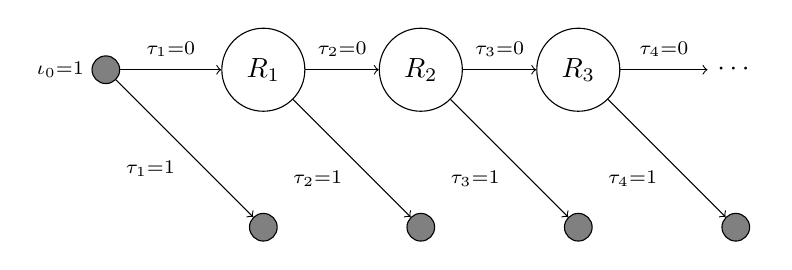
\begin{tikzpicture}[cnode/.style={draw,circle,minimum size=3em,inner sep=3pt}, onode/.style={fill=black!50, draw,circle,minimum size=1em}]
    \node (0i) at (-1,0) [right] {$\stackrel{\iota_0=1}{}$};
    \node[onode] (0) at (0,0) {};
    \node[cnode] (1) at (2,0) {$R_1$};
    \node[onode] (1t) at (2,-2) {};
    \node[cnode] (2) at (4, 0)  {$R_2$};
    \node[onode] (2t) at (4,-2) {};
    \node[cnode] (3) at (6, 0)  {$R_3$};
    \node[onode] (3t) at (6,-2) {};
    \node (t) at (8, 0) {$\cdots$};
    \node[onode] (tt) at (8, -2) {};

    \draw[->] (0) edge node [pos=0.5, above] {$\stackrel{\tau_1=0}{}$}  (1) ;
    \draw[->] (0) edge node [pos=0.5, below left] {$\stackrel{\tau_1=1}{}$} (1t) ;
    \draw[->] (1) edge node [pos=0.5, above] {$\stackrel{\tau_2=0}{}$}  (2) ;
    \draw[->] (1) edge node [pos=0.5, below left] {$\stackrel{\tau_2=1}{}$} (2t) ;
    \draw[->] (2) edge node [pos=0.5, above] {$\stackrel{\tau_3=0}{}$}  (3) ;
    \draw[->] (2) edge node [pos=0.5, below left] {$\stackrel{\tau_3=1}{}$} (3t) ;
    \draw[->] (3) edge node [pos=0.5, above] {$\stackrel{\tau_4=0}{}$}  (t) ;
    \draw[->] (3) edge node [pos=0.5, below left] {$\stackrel{\tau_4=1}{}$} (tt) ;
\end{tikzpicture}
\caption{\em A random process for generating complete sequences of arbitrary length,
with explicit stages for sequence initiation and termination. Multiple arrows exiting from a node indicate
different possible (mutually exclusive) stage transition pathways.}
\label{fig:random-process}
\end{figure}

The probability of a given complete sequence $\langle\vec{r}_n\rangle$ is now defined as
\begin{eqnarray}
   p(\langle\vec{r}_n\rangle)
& = & p(\iota_0\!=\!1,\tau_1\!=\!0,R_1=r_1,\ldots,\tau_n\!=\!0,R_n=r_n,\tau_{n+1}\!=\!1)
\,,
\end{eqnarray}
such that 
\begin{eqnarray}
   p(N\!=\!n) & = &  p(\iota_0\!=\!1,\tau_1\!=\!0,\ldots,\tau_n\!=\!0,\tau_{n+1}\!=\!1)\,.
\end{eqnarray}
This takes the form of a generalised Bernoulli sequence.
Likewise, the probability
of a given start sequence $\langle\vec{r}_n]$ is defined as
\begin{eqnarray}
p(\langle\vec{r}_n]) 
& = & p(\iota_0\!=\!1,\tau_1\!=\!0,R_1=r_1,\ldots,\tau_n\!=\!0,R_n=r_n)\,,
\end{eqnarray}
and the probability of the end sequence $[\vec{r}_n\rangle$ is
\begin{eqnarray}
p([\vec{r}_n\rangle)
& = & p(\tau_1\!=\!0,R_1=r_1,\ldots,\tau_n\!=\!0,R_n=r_n,\tau_{n+1}\!=\!1)\,.
\end{eqnarray}
In the special case where we know in advance that a start sequence definitely does not terminate
at stage $n+1$,  we may instead write
\begin{eqnarray}
p(\langle\vec{r}_n!)
& = & p(\iota_0\!=\!1,\tau_1\!=\!0,R_1=r_1,\ldots,\tau_n\!=\!0,R_n=r_n,\tau_{n+1}\!=\!0)\,.
\end{eqnarray}
Likewise, if an end sequence definitely does not initiate at stage 0, then
\begin{eqnarray}
p(!\vec{r}_n\rangle)
& = & p(\iota_0\!=\!0,\tau_1\!=\!0,R_1=r_1,\ldots,\tau_n\!=\!0,R_n=r_n,\tau_{n+1}\!=\!1)\,.
\end{eqnarray}
The four remaining types of sequences, namely $[\vec{r}_n]$, $!\vec{r}_n]$, $[\vec{r}_n!$ and $!\vec{r}_n!$ , can be similarly defined.

%%%%%%%%%%%%%%%%%%%%%%%%%%%%%%%%%%%
\section{Markov Sequence Processes}
\label{sec:markov-processes}
In Section~\ref{sec:random-processes} we defined a random process $R$ and the sequences it generates.
We now assume that the process is also {\em causal}, meaning that each stage of a sequence,
including the termination stage, depends only on the preceding stages.
This causal process, depicted in Figure~\ref{fig:causal-process}, is simply the random process from
Figure~\ref{fig:random-process} with additional, explicit dependencies (in the form of dashed arrows).
Hence, under the Markov assumption of conditional independence,
the causal sequence process leads to the fully-dependent, conditional model
\begin{eqnarray}
p(\langle\vec{r}_n\rangle) & = &
p(\iota_0=1)
\nonumber\\&&
{}\times \prod_{t=1}^{n}\left\{p(\tau_t\!=\!0\,|\,\iota_0\!=\!1,\vec{\tau}_{t-1}\!=\!\vec{0},\vec{R}_{t-1}\!=\!\vec{r}_{t-1})
\,p(R_t\!=\!r_t\,|\,\iota_0\!=\!1,\vec{\tau}_t\!=\!\vec{0},\vec{R}_{t-1}\!=\!\vec{r}_{t-1})\right\}
\nonumber\\&&
{}\times p(\tau_{n+1}\!=\!1\:|\;\iota_0\!=\!1,\vec{\tau}_n\!=\!\vec{0},\vec{R}_n\!=\!\vec{r}_n)
\,.
\label{eq:temporal-model}
\end{eqnarray}
The related models for partially complete or incomplete sequences can be similarly obtained
by suitably modifying the corresponding boundary conditions for $\iota_0$ and $\tau_{n+1}$
--- refer to Section~\ref{sec:random-processes}.
\begin{figure}[hbt]
\centering
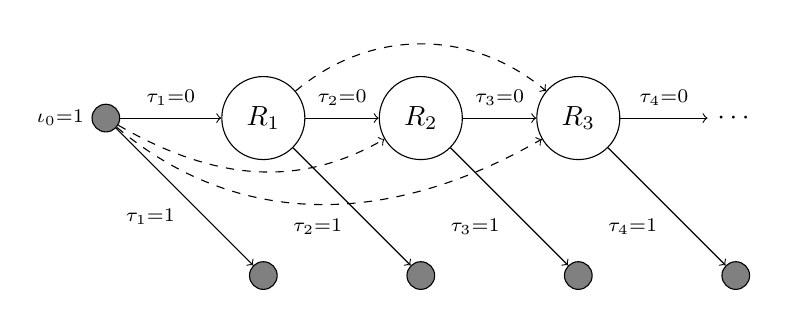
\begin{tikzpicture}[cnode/.style={draw,circle,minimum size=3em,inner sep=3pt}, onode/.style={fill=black!50, draw,circle,minimum size=1em}]
    \node (0i) at (-1,0) [right] {$\stackrel{\iota_0=1}{}$};
    \node[onode] (0) at (0,0) {};
    \node[cnode] (1) at (2,0) {$R_1$};
    \node[onode] (1t) at (2,-2) {};
    \node[cnode] (2) at (4, 0)  {$R_2$};
    \node[onode] (2t) at (4,-2) {};
    \node[cnode] (3) at (6, 0)  {$R_3$};
    \node[onode] (3t) at (6,-2) {};
    \node (t) at (8, 0) {$\cdots$};
    \node[onode] (tt) at (8, -2) {};

    \draw[->] (0) edge node [pos=0.5, above] {$\stackrel{\tau_1=0}{}$}  (1) ;
    \draw[->] (0) edge node [pos=0.5, below left] {$\stackrel{\tau_1=1}{}$} (1t) ;
    \draw[->] (1) edge node [pos=0.5, above] {$\stackrel{\tau_2=0}{}$}  (2) ;
    \draw[->] (1) edge node [pos=0.5, below left] {$\stackrel{\tau_2=1}{}$} (2t) ;
    \draw[->] (2) edge node [pos=0.5, above] {$\stackrel{\tau_3=0}{}$}  (3) ;
    \draw[->] (2) edge node [pos=0.5, below left] {$\stackrel{\tau_3=1}{}$} (3t) ;
    \draw[->] (3) edge node [pos=0.5, above] {$\stackrel{\tau_4=0}{}$}  (t) ;
    \draw[->] (3) edge node [pos=0.5, below left] {$\stackrel{\tau_4=1}{}$} (tt) ;

   \begin{scope}[dashed]
    \draw[->] (0) to[out=-30,in=-150] (2) ;
    \draw[->] (0) to[out=-40,in=-150] (3) ;
    \draw[->] (1) to[out=40,in=140] (3) ;
   \end{scope}
\end{tikzpicture}
\caption{\em A fully-dependent, causal process for generating complete sequences of arbitrary length.
Solid arrows indicate possible stage transitions.
Both dashed arrows and solid arrows indicate parent--child dependencies, such that the child node is conditionally dependent on the parent and all other previous nodes.}
\label{fig:causal-process}
\end{figure}


In practice, the causal model is usually simplified further by 
dropping some of the explicit (dashed) dependencies.
For example, one might limit the 
conditionality on past values to a maximum number $m$ of depenencies.
This leads to the so-called {\em $m$-th order Markov model}.
An example from the realm of natural language understanding is the lexicographical analysis of the character
sequences of words using bigrams (pairs of adjacent characters, corresponding to $m=1$), and trigrams 
(triples of adjacent characters, corresponding to $m=2$), et cetera.

In the special case of $m=1$, the first-order Markov model takes on the restricted conditional form
\begin{eqnarray}
p(\langle\vec{r}_n\rangle) & = &
p(\iota_0=1)\,p(\tau_1\!=\!0\,|\,\iota_0\!=\!1)
p(R_1\!=\!r_1\,|\,\iota_0\!=\!1,\tau_1\!=\!0)
\nonumber\\&&
{}\times\prod_{t=2}^{n}\left\{p(\tau_t\!=\!0\,|\,R_{t-1}\!=\!r_{t-1})
\,p(R_t\!=\!r_t\,|\,\tau_t\!=\!0,R_{t-1}\!=\!r_{t-1})\right\}
\nonumber\\&&
{}\times p(\tau_{n+1}\!=\!1\:|\;R_n\!=\!r_n)
\,.
\end{eqnarray}
This is just the strict Markov interpretation of the random process depicted in Figure~\ref{fig:random-process},
where each stage directly depends only on the previous stage {\em and} on the transition path between the two adjacent stages.

\section{Stateful Markov Sequence Processes}
Consider the first-order Markov process $R$ depicted in Figure~\ref{fig:random-process}.
Suppose now that the random variable $R_t$ at stage $t$ can be decomposed into the tuple
$R_t=(S_t,X_t)$, where $S_t$ is a random variable taking values $s_t\in{\cal S}$, and $X_t$
is a random variable taking values $x_t\in{\cal X}$.
We may call $S_t$ the {\em state} of the process at stage $t$, and $X_t$ its {\em value}.
As is usual, we presuppose that the stage transitions in the sequence generating process are primarily between states, e.g.\ from $S_{t-1}$ to $S_t$, 
and hence it follows that the value is generated after the state has been determined, i.e.\ $X_t$ depends upon $S_t$.
Keeping to the first-order Markov interpretation of stage-to-stage dependencies leads to
the {\em stateful} process depicted in Figure~\ref{fig:stateful-process}, with full cross-dependencies between $(S_t,X_t)$ and
$(S_{t+1},X_{t+1})$.
\begin{figure}[hbt]
\centering
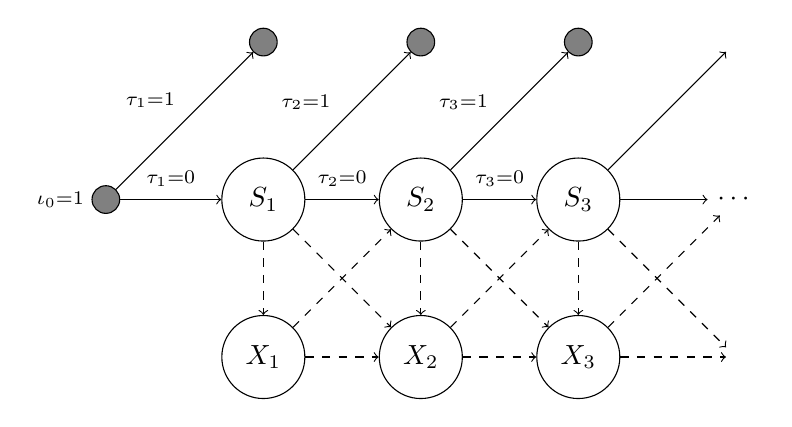
\begin{tikzpicture}[cnode/.style={draw,circle,minimum size=3em,inner sep=3pt}, onode/.style={fill=black!50, draw,circle,minimum size=1em}]
    \node (0i) at (-1,0) [right] {$\stackrel{\iota_0=1}{}$};
    \node[onode] (0) at (0,0) {};
    \node[cnode] (1) at (2,0) {$S_1$};
    \node[cnode] (1x) at (2,-2) {$X_1$};
    \node[onode] (1t) at (2,2) {};
    \node[cnode] (2) at (4, 0)  {$S_2$};
    \node[cnode] (2x) at (4, -2)  {$X_2$};
    \node[onode] (2t) at (4,2) {};
    \node[cnode] (3) at (6, 0)  {$S_3$};
    \node[cnode] (3x) at (6, -2)  {$X_3$};
    \node[onode] (3t) at (6,2) {};
    \node (t) at (8, 0) {$\cdots$};
    \node (tx) at (8, -2)  {};
    \node (tt) at (8,2) {};

    \draw[->] (0) edge node [pos=0.5, above] {$\stackrel{\tau_1=0}{}$}  (1) ;
    \draw[->] (0) edge node [pos=0.5, above left] {$\stackrel{\tau_1=1}{}$} (1t) ;
    \draw[->] (1) edge node [pos=0.5, above] {$\stackrel{\tau_2=0}{}$}  (2) ;
    \draw[->] (1) edge node [pos=0.4, above left] {$\stackrel{\tau_2=1}{}$} (2t) ;
    \draw[->] (2) edge node [pos=0.5, above] {$\stackrel{\tau_3=0}{}$}  (3) ;
    \draw[->] (2) edge node [pos=0.4, above left] {$\stackrel{\tau_3=1}{}$} (3t) ;
    \draw[->] (3) edge (t) ;
    \draw[->] (3) edge (tt) ;

   \begin{scope}[dashed]
    \draw[->] (1) to (1x) ;
    \draw[->] (1) to (2x) ;
    \draw[->] (1x) to (2) ;
    \draw[->] (1x) to (2x) ;
    \draw[->] (2) to (2x) ;
    \draw[->] (2) to (3x) ;
    \draw[->] (2x) to (3) ;
    \draw[->] (2x) to (3x) ;
    \draw[->] (3) to (3x) ;
    \draw[->] (3) to (tx) ;
    \draw[->] (3x) to (tx) ;
    \draw[->] (3x) to (t) ;
   \end{scope}
\end{tikzpicture}
\caption{\em A random process for generating complete, stateful  sequences of arbitrary length,
with explicit cross-dependencies between the states and values of adjacent stages.}
\label{fig:stateful-process}
\end{figure}

Hence, the fully-structured stateful model is now given by
\begin{eqnarray}
p(\iota_0,\vec{S}_n,\vec{X}_n,\vec{\tau}_{n+1}) & = & 
p(\iota_0)\,p(\tau_1\,|\,\iota_0)\,p(S_1\,|\,\iota_0,\tau_1)\,p(X_1\,|\,S_1)
\nonumber\\&&
{}\times\prod_{t=2}^{n}\left\{p(\tau_t\,|\,S_{t-1})\,p(S_t\,|\,\tau_t,S_{t-1},X_{t-1})
\,p(X_t\,|\,S_t,S_{t-1},X_{t-1})\right\}
\nonumber\\&&
{}\times p(\tau_{n+1}\,|\,S_n)
\,.
\end{eqnarray}
Conditioning the state $S_t$ on both the previous state $S_{t-1}$ and its value $X_{t-1}$
can be useful in some circumstances, e.g.\ in sequence classification problems.
However, due to the increased complexity of such models, it is more usual to further restrict the stateful process
by also imposing the first-order Markov assumption at the level
of the state--value dependencies themselves. In terms of the process depicted in Figure~\ref{fig:stateful-process},
this means retaining only direct node-to-node dependencies, rather than stage-to-stage dependencies.
Hence, this restricted process, depicted in Figure~\ref{fig:stateful-1-process},
corresponds to the sequence model
\begin{eqnarray}
p(\iota_0,\vec{S}_n,\vec{X}_n,\vec{\tau}_{n+1}) & = & 
p(\iota_0)\,p(\tau_1\,|\,\iota_0)\,p(S_1\,|\,\iota_0)\,p(X_1\,|\,S_1)
\nonumber\\&&
{}\times\prod_{t=2}^{n}\left\{p(\tau_t\,|\,S_{t-1})\,p(S_t\,|\,S_{t-1})\,p(X_t\,|\,S_t)\right\}
\,p(\tau_{n+1}\,|\,S_n)
\,.
\label{eq:stateful-1-model}
\end{eqnarray}
\begin{figure}[hbt]
\centering
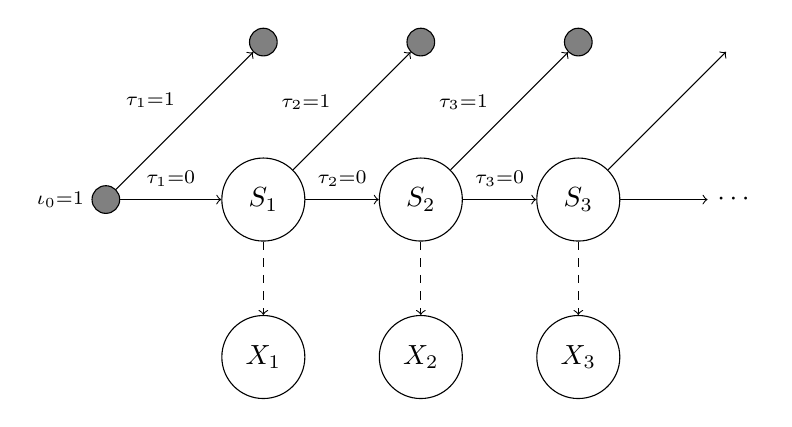
\begin{tikzpicture}[cnode/.style={draw,circle,minimum size=3em,inner sep=3pt}, onode/.style={fill=black!50, draw,circle,minimum size=1em}]
    \node (0i) at (-1,0) [right] {$\stackrel{\iota_0=1}{}$};
    \node[onode] (0) at (0,0) {};
    \node[cnode] (1) at (2,0) {$S_1$};
    \node[cnode] (1x) at (2,-2) {$X_1$};
    \node[onode] (1t) at (2,2) {};
    \node[cnode] (2) at (4, 0)  {$S_2$};
    \node[cnode] (2x) at (4, -2)  {$X_2$};
    \node[onode] (2t) at (4,2) {};
    \node[cnode] (3) at (6, 0)  {$S_3$};
    \node[cnode] (3x) at (6, -2)  {$X_3$};
    \node[onode] (3t) at (6,2) {};
    \node (t) at (8, 0) {$\cdots$};
    \node (tx) at (8, -2)  {};
    \node (tt) at (8,2) {};

    \draw[->] (0) edge node [pos=0.5, above] {$\stackrel{\tau_1=0}{}$}  (1) ;
    \draw[->] (0) edge node [pos=0.5, above left] {$\stackrel{\tau_1=1}{}$} (1t) ;
    \draw[->] (1) edge node [pos=0.5, above] {$\stackrel{\tau_2=0}{}$}  (2) ;
    \draw[->] (1) edge node [pos=0.4, above left] {$\stackrel{\tau_2=1}{}$} (2t) ;
    \draw[->] (2) edge node [pos=0.5, above] {$\stackrel{\tau_3=0}{}$}  (3) ;
    \draw[->] (2) edge node [pos=0.4, above left] {$\stackrel{\tau_3=1}{}$} (3t) ;
    \draw[->] (3) edge (t) ;
    \draw[->] (3) edge (tt) ;

   \begin{scope}[dashed]
    \draw[->] (1) to (1x) ;
    \draw[->] (2) to (2x) ;
    \draw[->] (3) to (3x) ;
   \end{scope}
\end{tikzpicture}
\caption{\em A first-order Markov process for generating complete, stateful  sequences of arbitrary length.}
\label{fig:stateful-1-process}
\end{figure}

\section{Discrete-state Sequence Models}

Consider the stateful, first-order Markov process depicted by Figure~\ref{fig:stateful-1-process}.
Let us now restrict our attention to the class of models where
the state $S_t$ at any stage $t$ may now only take {\em discrete} values in the set ${\cal S}=\{\sigma_1,\sigma_2,\ldots,\sigma_S\}$.
Thus, the sequence model~\eqref{eq:stateful-1-model} may be parameterised in terms of arbitrary states $\vec{s}_n=(\sigma_{i_1},\sigma_{i_2},\ldots,\sigma_{i_n})$,
where the factors modelling the probabilities within stage $t$ depend only upon $\sigma_{i_t}$, and the factors modelling the transition between stage $t$ and stage $t+1$ 
depend only upon $\sigma_{i_t}$ and $\sigma_{i_{t+1}}$.
For convenience, let us further assume that the process does not generate zero-length sequences\footnote{Zero-length sequences are usually undetectable in practice,
unless the generating process explicitly indicates the start and end of such sequences. Even if clearly delimited, zero-length sequences may typically be ignored in
most applications.}, so that $p(\tau_1=1\,|\,\iota_0=1)=1$.
Consequently, model~\eqref{eq:stateful-1-model} can now be explicitly rewritten in terms of the parameters $\theta=(\vec{\pi},\vec{\bar{\pi}},\Gamma,\vec{\omega})$, 
such that the probability of an arbitrary, complete sequence is given by
\begin{eqnarray}
\hspace*{-5mm}
p(\langle\vec{s},\vec{x}\rangle\,|\,\theta) & = & \pi_{1,i_1}\,o_{1,i_1}(x_1)\left\{\prod_{t=1}^{n-1}\bar{\omega}_{t,i_t}\,\Gamma_{t,i_t,i_{t+1}}\,o_{t,i_{t+1}}(x_{t+1})
\right\}\,\omega_{n,i_n}
\,,
\label{eq:p_s_x_g_theta}
\end{eqnarray}
where $n=|\vec{x}|=|\vec{s}|$.
The initial state $S_1$ of the sequence at stage $t=1$ is governed by the general parameter
\begin{eqnarray}
  \pi_{t,i} & = & p(\iota_{t-1}\!=\!1\,|\,\theta)\,p(S_t\!=\!\sigma_{i}\,|\,\iota_{t-1}\!=\!1,\theta)\,,
\end{eqnarray}
and the terminal and non-terminal transitions between stages $t$ and $t+1$ are governed by
\begin{eqnarray}
  \omega_{t,i} & = & p(\tau_{t+1}=1\,|\,S_t\!=\!\sigma_{i},\theta)\,,
\\
  \bar{\omega}_{t,i} & = & p(\tau_{t+1}=0\,|\,S_t\!=\!\sigma_{i},\theta)~=~1-\omega_{t,i}\,,
\end{eqnarray}
respectively. The possible transitions between the states $S_t$ and $S_{t+1}$ of consecutive stages $t$ and $t+1$ are governed by
\begin{eqnarray}
  \Gamma_{t,i,j} & = & p(S_{t+1}\!=\!\sigma_{j}\,|\,S_t\!=\!\sigma_{i},\theta)\,.
\end{eqnarray}
Clearly, a state transition from $S_t$ to $S_{t+1}$ implies a non-terminal transition from stage $t$ to $t+1$ in the sequence. 
This is explicitly modelled by the presence of the $\bar{\omega}_{t,i_t}$ term,
which is interpreted to mean that $S_t$ is a non-terminal state.
It then follows that $S_{t+1}$ is a non-initial state which, if modelled explicitly, would be represented by a corresponding $\bar{\pi}_{t+1,i_{t+1}}$ term, defined by
\begin{eqnarray}
  \bar{\pi}_{t,i} & = & p(\iota_{t-1}\!=\!0\,|\,\theta)\,p(S_{t}\!=\!\sigma_{i}\,|\,\iota_{t-1}\!=\!0,\theta)\,.
\end{eqnarray}
However, $\bar{\pi}_{t+1,i_{t+1}}$ is already implicit the explicit transition term $\Gamma_{t,i_t,i_{t+1}}$,
since we cannot count state $S_{t+1}$ twice. This fact is important when it comes to parameter estimation (see Section~\ref{sec:param-estimation}).

Lastly, the probabilities of observed values at stage $t$ are governed by
\begin{eqnarray}
  o_{t,i}(x) & = & p(X_t\!=\!x\,|\,S_t\!=\!\sigma_{i},\theta) \hspace*{5mm}\forall x\in{\cal X}\,.
\end{eqnarray}
We do not, however, explicitly declare the parameterisation structure of this likelihood model (see Section~\ref{sec:discrete-x} for a plausible model if $X_t$ takes discrete values). 
It suffices for our calculations that each $o_{t,i_t}(x_t)$ is available when required.

Note that all other types of incomplete sequences (see Section~\ref{sec:random-processes}) are handled similarly to complete sequences by modifying the first and/or last terms of model~\eqref{eq:p_s_x_g_theta}.
For example, $!\vec{s},\vec{x}\rangle$ is modelled by replacing $\pi_{1,i_1}$ by $\bar{\pi}_{1,i_1}$, whereas $[\vec{s},\vec{x}\rangle$ is modelled by replacing $\pi_{1,i_1}$ by $\breve{\pi}_{1,i_1}$, where
\begin{eqnarray}
  \breve{\pi}_{t,i} & = & \pi_{t,i}+\bar{\pi}_{t,i}
\nonumber\\& = &
  p(\iota_{t-1}\!=\!1)\,p(S_t\!=\!\sigma_{i}\,|\,\iota_{t-1}\!=\!1,\theta)
+
  p(\iota_{t-1}\!=\!0)\,p(S_t\!=\!\sigma_{i}\,|\,\iota_{t-1}\!=\!0,\theta)
\nonumber\\& = &
  p(\iota_{t-1}\!=\!1,S_t\!=\!\sigma_{i}\,|\,\theta)
+
  p(\iota_{t-1}\!=\!0,S_t\!=\!\sigma_{i}\,|\,\theta)
\nonumber\\& = &
  p(S_t\!=\!\sigma_{i}\,|\,\theta)\,.
\end{eqnarray}
Similarly, $\langle\vec{s},\vec{x}!$ is modelled by replacing $\omega_{n,i_{n}}$ by $\bar{\omega}_{n,i_{n}}$, whereas $\langle\vec{s},\vec{x}]$ 
is modelled by replacing $\omega_{n,i_n}$ by $\breve{\omega}_{n,i_n}$, where
\begin{eqnarray}
   \breve{\omega}_{t,i} & = & \omega_{t,i}+\bar{\omega}_{t,i}
\nonumber\\& = &
   p(\tau_{t+1}\!=\!1\,|\,S_t\!=\!\sigma_i,\theta) + p(\tau_{t+1}\!=\!0\,|\,S_t\!=\!\sigma_i,\theta)
\nonumber\\& = &
  1\,.
\end{eqnarray}

\subsection{Posterior State Prediction}

A {\em hidden-state} Markov model (or HMM) results from a stateful Markov sequence process like Figure~\ref{fig:stateful-1-process}, from which the values $\vec{x}$ are observed
but the states $\vec{s}$ are not. The true state values are then said to be {\em missing} or {\em hidden}, and must be estimated from the observed data.
In particular, a known problem is to deduce the state $S_t$ given $\vec{x}$, at each stage $t=1,2,\ldots,n$. This is accomplished
via the {\em forward--backward algortithm}, which uses the causal nature of the process to notionally partitition the sequence into past and present stages $1,2,\ldots,t$ and future stages $t+1,t+2,\ldots,n$.
The standard algorithm is modified here to include the stage-by-stage probabilities of sequence termination.
Thus, the posterior state probabilities at stage $t$ for a complete sequence $\langle\vec{x}\rangle$ are given by
\begin{eqnarray}
   \gamma_{t,i} & = & p(S_t\!=\!\sigma_i\,|\,\langle\vec{x}\rangle,\theta)
\nonumber\\& = &
   \frac{p(S_t\!=\!\sigma_i,\langle\vec{x}\rangle\,|\,\theta)}
        {p(\langle\vec{x}\rangle\,|\,\theta)}
\nonumber\\& = &
   \frac{p(S_t\!=\!\sigma_i,\langle\vec{x}_t]\,|\,\theta)\,p([\rvec{x}_{t+1}\rangle\,|\,S_t\!=\!\sigma_i,\theta)}
        {\sum_{i'=1}^{S}p(S_t\!=\!\sigma_{i'},\langle\vec{x}_t]\,|\,\theta)\,p([\rvec{x}_{t+1}\rangle\,|\,S_t\!=\!\sigma_{i'},\theta)}
\nonumber\\& = &
   \frac{\alpha_{t,i}\,\beta_{t,i}}
        {\sum_{i'=1}^{S}\alpha_{t,i}\,\beta_{t,i}}
\,,
\label{eq:gamma_t_i}
\end{eqnarray}
where we have defined $\rvec{x}_{t}=(x_t,x_{t+1},\ldots,x_n)$ for all $t=1,2,\ldots,n$, with $n=|\vec{x}|$.

The {\em forward step}, which incorporates information about the initiation of the sequence, is recursively defined via
\begin{eqnarray}
   \alpha_{t,i} & = & p(S_t\!=\!\sigma_i,\langle\vec{x}_t]\,|\,\theta)
\nonumber\\& = &
   \sum_{j=1}^{S}p(S_{t-1}\!=\!\sigma_j,\langle\vec{x}_{t-1}]\,|\,\theta)
      \,p(\tau_t\!=\!0\,|\,S_{t-1}\!=\!\sigma_j,\theta)
\nonumber\\&&
    \hspace*{5mm}{}\times\,p(S_t\!=\!\sigma_i\,|\,S_{t-1}\!=\!\sigma_j,\theta)\,p(X_t\!=\!x_t\,|\,S_t\!=\!\sigma_i,\theta)
\nonumber\\& = &
   \left\{\sum_{j=1}^{S}\alpha_{t-1,j}\,\bar{\omega}_{t-1,j}\,\Gamma_{t-1,j,i}\right\}\,o_{t,i}(x_t)\,,
\end{eqnarray}
for $t=2,3,\ldots,n$. The forward step commences with
\begin{eqnarray}
  \alpha_{1,i} & = & p(S_1\!=\!\sigma_i,\langle x_1]\,|\,\theta)
\nonumber\\& = & 
  p(\iota_0\!=\!1)\,p(S_1\!=\!\sigma_i\,|\,\iota_0\!=\!1,\theta)\,p(X_1\!=\!x_1\,|\,S_1\!=\!\sigma_i,\theta)
\nonumber\\& = & 
  \pi_{1,i}\,o_{1,i}(x_1)
\,.
\end{eqnarray}
Note that incompletely--initiated sequences such as $!\vec{x}]$ and $[\vec{x}]$ can also be handled by substituting $\bar{\pi}$ and $\breve{\pi}$ for $\pi$ in $\alpha$, thereby obtaining
$\bar{\alpha}$ and $\breve{\alpha}$ respectively.

Consequently, we may predict $S_t$ from a partially observed sequence $\langle\vec{x}_t]$ via
\begin{eqnarray}
  p(S_t\!=\!\sigma_i\,|\,\langle\vec{x}_t],\theta) & = & 
  \frac{p(S_t\!=\!\sigma_i,\langle\vec{x}_t]\,|\,\theta)}
       {\sum_{i'=1}^{S}p(S_t\!=\!\sigma_{i'},\langle\vec{x}_t]\,|\,\theta)}
\nonumber\\& = & 
  \frac{\alpha_{t,i}}{\sum_{i'=1}^{S}\alpha_{t,i'}}\,.
\end{eqnarray}
Similarly, we may predict the next observation $X_{t+1}$ via
\begin{eqnarray}
  p(X_{t+1}\!=\!x\,|\,\langle\vec{x}_t],\theta) 
& = &
  \frac{p(\langle\vec{x}_{t},x]\,|\,\theta)}
       {p(\langle\vec{x}_{t}]\,|\,\theta)}
\nonumber\\& = & 
  \frac{\sum_{j=1}^S p(S_{t+1}\!=\!\sigma_j,\langle\vec{x}_{t},x]\,|\,\theta)}
       {\sum_{i=1}^S p(S_{t}\!=\!\sigma_i,\langle\vec{x}_{t}]\,|\,\theta)}
\nonumber\\& = & 
  \frac{\sum_{j=1}^S\left\{\sum_{i=1}^S\alpha_{t,i}\,\bar{\omega}_{t,i}\,\Gamma_{t,i,j}\right\}o_{t+1,j}(x)}
       {\sum_{i=1}^S\alpha_{t,i}}
\,.
\end{eqnarray}

The {\em backward step}, which incorporates information about the termination of the sequence, is now also recursively defined via
\begin{eqnarray}
   \beta_{t,i} & = & p([\rvec{x}_{t+1}\rangle\,|\,S_t\!=\!\sigma_i,\theta)
\nonumber\\& = & 
   \sum_{j=1}^{S}p([\rvec{x}_{t+2}\rangle\,|\,S_{t+1}\!=\!\sigma_j,\theta)\,p(X_{t+1}=x_{t+1}\,|\,S_{t+1}\!=\!\sigma_j,\theta)
\nonumber\\&& \hspace*{5mm}{}\times
       p(S_{t+1}\!=\!\sigma_j\,|\,S_t\!=\!\sigma_i,\theta)\,p(\tau_{t+1}\!=\!0\,|\,S_t\!=\!\sigma_i,\theta)
\nonumber\\& = & 
	\left\{\sum_{j=1}^{S}\beta_{t+1,j}\,o_{t+1,j}(x_{t+1})\,\Gamma_{t,i,j}\right\}\,\bar{\omega}_{t,i}
\,,
\end{eqnarray}
for $t=n-1,n-2,\ldots,1$. The backward step commences with
\begin{eqnarray}
   \beta_{n,i} & = & p(\tau_{n+1}\!=\!1\,|\,S_n\!=\!\sigma_i,\theta)~=~\omega_{n,i}\,.
\end{eqnarray}
Note that incompletely--terminated sequences such as $[\vec{x}!$ and $[\vec{x}]$ can also be handled by substituting $\bar{\omega}$ and $\breve{\omega}$ for $\omega$ in $\beta$, thereby obtaining
$\bar{\beta}$ and $\breve{\beta}$ respectively.

The combination of the forward step with the backward step now enables us to use all of the information contained in the observed sequence, including its possible initiation and/or termination.
Particularly, we can compute the joint probability of any observed sequence, as a prelude to estimating the state of each stage
from equation~\eqref{eq:gamma_t_i}. For example, observe that
\begin{eqnarray}
   p(\langle\vec{x}!\,|\,\theta) 
& = &
	\sum_{i=1}^{S}p(S_t\!=\!\sigma_i,\langle\vec{x}!\,|\,\theta)
\nonumber\\& = &
   \sum_{i=1}^{S}p(S_t\!=\!\sigma_i,\langle\vec{x}_t]\,|\,\theta)\,p([\rvec{x}_{t+1}!\,|\,S_t\!=\!\sigma_i,\theta) 
\nonumber\\& = &
   \sum_{i=1}^{S}\alpha_{t,i}\bar{\beta}_{t,i}\,,
\end{eqnarray}
for all $t=1,2,\ldots,n$.

Finally, the forward--backward calculations also enable us to compute the posterior probabilities of the joint states of stages $t$ and $t+1$.
For example, given the observed, complete sequence $\langle\vec{x}\rangle$, we obtain
\begin{eqnarray}
\xi_{t,i,j} & = &
   p(S_t\!=\!\sigma_i,S_{t+1}\!=\!\sigma_j\,|\,\langle\vec{x}\rangle,\theta)
\nonumber\\& = & 
   \frac{p(S_t\!=\!\sigma_i,S_{t+1}\!=\!\sigma_j,\langle\vec{x}\rangle\,|\,\theta)}
        {p(\langle\vec{x}\rangle\,|\,\theta)}
\,,
\label{eq:xi_t_i_j}
\end{eqnarray}
where
\begin{eqnarray}
   p(S_t\!=\!\sigma_i,S_{t+1}\!=\!\sigma_j,\langle\vec{x}\rangle\,|\,\theta)
& = & 
   p(S_t\!=!\sigma_i,\langle\vec{x}_t]\,|\,\theta)
     \,p(\tau_{t+1}\!=\!0\,|\,S_t\!=\!\sigma_i,\theta)
\nonumber\\&&{}\times
     \,p(S_{t+1}\!=\!\sigma_j\,|\,S_t\!=\!\sigma_i,\theta)
	 \,p([\rvec{x}_{t+1}]\,|\,S_{t+1}\!=\!\sigma_j,\theta)
\nonumber\\& = & 
   \alpha_{t,i}\,\bar{\omega}_{t,i}\,\Gamma_{t,i,j}\,\beta_{t+1,j}
\,,
\end{eqnarray}
and thus
\begin{eqnarray}
   p(\langle\vec{x}\rangle\,|\,\theta)
& = &
   \sum_{i'=1}^{S}\sum_{j'=1}^{S}p(S_t\!=\!\sigma_i,S_{t+1}\!=\!\sigma_j,\langle\vec{x}\rangle\,|\,\theta)
\nonumber\\& = & 
   \sum_{i'=1}^{S}\sum_{j'=1}^{S}\alpha_{t,i'}\,\bar{\omega}_{t,i'}\,\Gamma_{t,i',j'}\,\beta_{t+1,j'}
\nonumber\\& = & 
   \sum_{i'=1}^{S}\alpha_{t,i'}\,\beta_{t,i'}
\,,
\end{eqnarray}
as expected.

\subsection{Modelling Observed Data}

%Suppose that we have observed an ordered set of sequences $\XX=\{\vec{v}^{(d)}\}_{d=1}^{D}$,
Suppose that we have observed an ordered set of sequences $\XX=\{\vec{v}^{(d)}\}_{d=1}^{D}$,
where each observation takes the form of $\vec{v}^{(d)}=(\iota^{(d)},\vec{s}^{(d)},\vec{x}^{(d)},\tau^{(d)})$.
Here $\iota^{(d)}$ takes one of the values $0$, $1$, or $*$, corresponding to the sequence initiation marker $\langle$, $!$ or $[$, respectively.
Note that $\iota^{(d)}=*$ is taken to mean that the true value of $\iota_0$ is unknown.
Similarly, $\tau^{(d)}$ takes one of the values $0$, $1$, or $*$, corresponding to the sequence termination marker $\rangle$, $!$ or $]$, respectively,
where $\tau^{(d)}=*$ means that the true value of $\tau_{|\vec{x}^{(d)}|+1}$ is unknown.
The observed values $\vec{x}^{(d)}$ are assumed to be known and to form a non-empty, contiguous sequence (or sub-sequence).
Hence, we may always assume here that $\vec{\tau}_{|\vec{x}^{(d)}|}=\vec{0}$.
Finally, the values of the state sequence $\vec{s}^{(d)}$ might or might not be specified.
In some circumstances, $\vec{s}^{(d)}$ is known; in others, some or all of these states might remain hidden.

In order to model the ambiguities that might be present in $\vec{v}^{(d)}$, we need some notation.
For convenience, we define the data-specified initial state distribution of the $d$-th observation as
\begin{eqnarray}
  \pi^{(d)}_{1,i} & = & \pi_{1,i}\delta(\iota_0^{(d)}=1)+\bar{\pi}_{1,i}\delta(\iota_0^{(d)}=0)\,,
\end{eqnarray}
where $\delta(\cdot)=1$ (or $0$) if its argument is true (or false). Note that $\iota^{(d)}=*$ is taken to match both $\iota_0=1$ and $\iota_0=0$.
Similarly, we define the data-specified terminal state distribution of the $d$-th observation as
\begin{eqnarray}
  \omega^{(d)}_{1,i} & = & \omega_{1,i}\delta(\iota_0^{(d)}=1)+\bar{\omega}_{1,i}\delta(\iota_0^{(d)}=0)\,.
\end{eqnarray}
Finally, if the state $S_t$ of stage $t$ is known, then we define $s^{(d)}_t=\sigma_{i_t^{(d)}}$, for $i^{(d)}_t\in\{1,2,\ldots,S\}$.
Otherwise, we define both $s^{(d)}_t=*$ and $i^{(d)}_t=*$.
Hence, from model~\eqref{eq:p_s_x_g_theta}, we obtain
\begin{eqnarray}
   p(\vec{v}^{(d)}\,|\,\theta) 
& = & 
   \sum_{i_1=1}^{S}\delta(i_1^{(d)}\!=\!i_1)\cdots\sum_{i_n^{(d)}=1}^{S}\delta(i_{n^{(d)}}^{(d)}\!=\!i_{n^{(d)}})

\end{eqnarray}
where we have marginalised over any missing data.

********************
Notionally, we may also define the correspondingly ordered set $\SS=\{\vec{s}^{(d)}\}_{d=1}^D$
of arbitrary state sequences.
Hence, under the assumption that the observed sequences are independent, the joint log-likelihood of the data is given by
\begin{eqnarray}
  L(\theta) & = & \log p(\SS,\XX\,|\,\theta) 
\nonumber\\& = & 
\log\prod_{d=1}^D 
p(\iota_0^{(d)},\vec{s}^{(d)},\vec{x}^{(d)},\tau_{n^{(d)}+1}^{(d)}\,|\,\theta) 
\nonumber\\& = & 
\sum_{d=1}^D\log 
p(\iota_0^{(d)},\vec{s}^{(d)},\vec{x}^{(d)},\tau_{n^{(d)}+1}^{(d)}\,|\,\theta) 
\nonumber\\& = & 
\sum_{d=1}^D L^{(d)}(\theta)
\,,
\end{eqnarray}
where
\begin{eqnarray}
  L^{(d)}(\theta) & = &
   \log\pi_{i_1^{(d)}}^{(d)}
 + \sum_{t=1}^{n^{(d)}-1}\log\Gamma_{i_t^{(d)},i_{t+1}^{(d)}}
 + \sum_{t=1}^{n^{(d)}}\log o_{t,i_t^{(d)}}
 + \log\omega_{i_{n^{(d)}}^{(d)}}^{(d)}
\,,
\end{eqnarray}
and $n^{(d)}=|\vec{x}^{(d)}|$.

However, recall that $\SS$ is actually uknown. Hence, we take an expectation of the log-likelihood over all possible values of
$\SS$, namely\footnote{Other expectations are possible, e.g.\ over the joint distribution $\SS,\XX\,|\,\theta$. This latter produces macro-averaged
parameter estimates of the form $\sum_{d=1}^D\phi^{(d)}/\sum_{d=1}^D\psi^{(d)}$, whereas the discriminative distribution $\SS\,|\,\XX,\theta$
often leads to micro-averaged estimates of the form $\sum_{d=1}^D\phi^{(d)}/\psi^{(d)}/D$.}
\begin{eqnarray}
  Q(\theta) & = & E_{\SS\,|\,\XX,\theta}\left[\log p(\SS,\XX\,|\,\theta)\right]
\nonumber\\& = & 
E_{\SS\,|\,\XX\theta}\left[
\sum_{d=1}^D L^{(d)}(\theta)
\right]
\nonumber\\& = & 
\sum_{d=1}^D E_{\SS\,|\,\XX,\theta}\left[
L^{(d)}(\theta)
\right]
\nonumber\\& = & 
\sum_{d=1}^D \sum_{i_1^{(d)}=1}^{S}\cdots\sum_{i^{(d)}_{n^{(d)}}}^{S}
p(\vec{s}^{(d)}\,|\,\iota_0^{(d)},\vec{x}^{(d)},\tau_{n^{(d)}+1}^{(d)},\theta) 
\,L^{(d)}(\theta)
\,.
\end{eqnarray}
In practice, it is difficult to optimise this nonlinear expression analytically. A feasible alternative is to iteratively apply the {\em expectation--maximisation}
(EM) algorithm:
\begin{enumerate}
\item {\em Expectation step:} Compute the expected log-likelihood conditioned on a known parameter estimate $\hat{\theta}_k$,
namely
\begin{eqnarray}
  Q(\theta,\hat{\theta}_k) & = & E_{\SS\,|\,\XX,\hat{\theta}_k}\left[\log p(\SS,\XX\,|\,\theta)\right]
\nonumber\\& = &
\sum_{d=1}^D \sum_{i_1^{(d)}=1}^{S}\cdots\sum_{i^{(d)}_{n^{(d)}}}^{S} 
p(\vec{s}^{(d)}\,|\,\iota_0^{(d)},\vec{x}^{(d)},\tau_{n^{(d)}+1}^{(d)},\hat{\theta}_k)
\,L^{(d)}(\theta)\,.
\end{eqnarray}

\item {\em Maximisation step:} Obtain the optimal parameter estimate $\hat{\theta}_{k+1}$ that maximises the
conditional expected log-likehood, namely
\begin{eqnarray}
\hat{\theta}_{k+1} & = & \arg\max_{\theta} Q(\theta,\hat{\theta}_k)\,.
\end{eqnarray}
\end{enumerate}
These two steps are iterated until $\hat{\theta}_k$ has converged to a value $\hat{\theta}^*$ that maximises 
$L(\hat{\theta}^*)=Q(\hat{\theta}^*,\hat{\theta}^*)$.

blah about additivity

\begin{eqnarray}
  \frac{\partial Q}{\partial\Gamma_{i,j}} & = & 
  \frac{\partial}{\partial\Gamma_{i,j}}
  \sum_{d=1}^D
  \sum_{i_1^{(d)}=1}^{S}\cdots\sum_{i^{(d)}_{n^{(d)}}}^{S} 
  p(\vec{s}^{(d)}\,|\,\iota_0^{(d)},\vec{x}^{(d)},\tau_{n^{(d)}+1}^{(d)},\hat{\theta}')
  \sum_{t=1}^{n^{(d)}-1}\log\Gamma_{i_t^{(d)},i_{t+1}^{(d)}}
\nonumber\\& = &
  \sum_{d=1}^D
  \sum_{t=1}^{n^{(d)}-1}
  \sum_{i_1^{(d)}=1}^{S}\cdots\sum_{i^{(d)}_{n^{(d)}}}^{S} 
  \delta(i^{(d)}_t=i)\delta(i^{(d)}_{t+1}=j)
  \frac{p(\vec{s}^{(d)}\,|\,\iota_0^{(d)},\vec{x}^{(d)},\tau_{n^{(d)}+1}^{(d)},\hat{\theta}')}
  {\Gamma_{i,j}}
\nonumber\\& = &
  \sum_{d=1}^D
  \sum_{t=1}^{n^{(d)}-1}
  \sum_{i_1^{(d)}=1}^{S}\cdots\sum_{i^{(d)}_{n^{(d)}}}^{S} 
  \delta(i^{(d)}_t=i)\delta(i^{(d)}_{t+1}=j)
  \frac{p(\vec{s}^{(d)}\,|\,\iota_0^{(d)},\vec{x}^{(d)},\tau_{n^{(d)}+1}^{(d)},\hat{\theta}')}
  {\Gamma_{i,j}}
\nonumber\\& = &
  \frac{\sum_{d=1}^D\sum_{t=1}^{n^{(d)}-1}p(S_t=\sigma_i,S_{t+1}=\sigma_j\,|\,\iota_0^{(d)},\vec{x}^{(d)},\tau_{n^{(d)}+1}^{(d)},\hat{\theta}')}
  {\Gamma_{i,j}}
\nonumber\\& = &
  \frac{\sum_{d=1}^D\sum_{t=1}^{n^{(d)}-1} \xi_t^{(d)}(\sigma_i,\sigma_j;\hat{\theta}')}
  {\Gamma_{i,j}}
\end{eqnarray}
from equation~\eqref{eq:xi-def}. Now, subject to the constraint that $\sum_{j=1}^{S}\Gamma_{i,j}=1$, we induce the appropriate Lagrangian multiplier to
provide the proper normalisation, and hence derive that the optimal parameter estimate is given by
\begin{eqnarray}
  \hat{\Gamma}^*_{i,j} & = &
  \frac{\sum_{d=1}^D\sum_{t=1}^{n^{(d)}-1} \xi_t^{(d)}(\sigma_i,\sigma_j;\hat{\theta}')}
  {\sum_{j=1}^{S}\sum_{d=1}^D\sum_{t=1}^{n^{(d)}-1} \xi_t^{(d)}(\sigma_i,\sigma_j;\hat{\theta}')}
~=~
  \frac{\sum_{d=1}^D\sum_{t=1}^{n^{(d)}-1} \xi_t^{(d)}(\sigma_i,\sigma_j;\hat{\theta}')}
  {\sum_{d=1}^D\sum_{t=1}^{n^{(d)}-1} \gamma_t^{(d)}(\sigma_i;\hat{\theta}')}
\end{eqnarray}
from equation~\eqref{eq:gamma-def}.

%%%%%%%%%%%%%%%%%%%%%%%%%%%%%%%%%%%%
\end{document}
